\section{Flujometrías y CFD}
%
Se realizó una serie de flujometrías para obtener valores de $C_{D}$ en función
de la diferencia de presión que \emph{ve} el puerto y la apertura del
mismo\footnote{ICESym utiliza alzada, por lo que se traduce área de pasaje de
puerto en alzada de válvula equivalente.}, con el fin de obtener un mapa en
función de la presión y la alzada $C_{D} = f(\Delta P,l_v)$.
%
ICESym requiere de información sobre el $C_{D}$ para calcular el área efectiva
de pasaje de flujo de las válvulas (o puertos en el caso del MRCVC),
introduciendo el mapa de $C_{D}$ se tiene un mejor modelado del funcionamiento
del sistema de intercambio de gases porque se conoce la pérdida de carga
localizada para un rango de operación del motor.

\subsection{Modelos de turbulencia}
%
El flujo a través del puerto es de carácter transitorio, turbulento; para
modelar este tipo de flujo se utilizó el modelo de turbulencia de dos ecuaciones
\emph{$\kappa-\epsilon$}\parencite{wilcox}, que brinda una ecuación para la
\emph{energía cinética turbulenta} $\kappa$ y otra para la \emph{velocidad de
disipación de la energía cinética turbulenta} $\epsilon$.
%
El modelo está basado en el modelo estándar
$\kappa-\epsilon$~\parencite{launderSpalding} y es uno de los más populares con
\emph{performance} conocida, las ecuaciones del modelo son:

\begin{equation}\label{eq:k}
  \frac{D}{Dt}(\rho \kappa) = \nabla \cdot (\rho D_{\kappa}\nabla \kappa) + P - \rho \epsilon
\end{equation}

Dónde:
\begin{itemize}
  \item[-] $\kappa$ es la energía cinética turbulente en $m^{2}s^{-2}$.
  \item[-] $D_{\kappa}$ es la difusividad efectiva para $\kappa$.
  \item[-] $P$ es la velocidad de producción de energía cinética turbulenta en $m^{2}s^{-3}$.
  \item[-] $\epsilon$ es la velocidad de disipación de energía cinética turbulenta en $m^{2}s^{-3}$.
\end{itemize}


\begin{equation}\label{eq:k}
  \frac{D}{Dt}(\rho \epsilon) = \nabla \cdot (\rho D_{\epsilon}\nabla \epsilon) \frac{C_{1}\epsilon}{\kappa} \left( P+C_{3}\frac{2}{3}\kappa\nabla\cdot u \right) - C_{2}\rho\frac{\epsilon^{2}}{\kappa}
\end{equation}

Dónde:
\begin{itemize}
  \item[-] $D_{\epsilon}$ es la difusividad efectiva de $\epsilon$.
  \item[-] $C_{1}$ es un coeficiente del modelo.
  \item[-] $C_{2}$ es un coeficiente del modelo.
\end{itemize}

La ecuación para la viscosidad turbulenta $\nu_{t}$ es

\begin{equation}\label{eq:nu_t}
  \nu_{t} = C_{\mu}\frac{\kappa^{2}}{\epsilon}
\end{equation}

Dónde:
\begin{itemize}
        \item[-] $C_{mu}$ es un coeficiente del modelo.
        \item[-] $\nu_{t}$ es la viscosidad turbulente en $m^{2}s^{-1}$.
\end{itemize}

Los coeficientes por defecto del modelo son

% Clossure Coefficient
\begin{equation}
  C_{\epsilon 1}=1.44
  \quad
  C_{\epsilon 2}=1.92
  \quad
  C_{\mu}=0.09
  \quad
  \sigma_{k}=1
  \quad
  \sigma_{\epsilon}=1.3
\end{equation}

El valor inicial para $\kappa$ se puede estimar con:
\begin{equation}\label{eq:kappa_est}
  \kappa = \frac{3}{2} {\left( |u_{ref}| \cdot I \right)}^{2}
\end{equation}

Dónde:
\begin{itemize}
  \item[-] $I$ es la intensidad de turbulencia en \%.
  \item[-] $u_{ref}$ es una velocidad de referencia en $ms^{-1}$.
\end{itemize}

El valor inicial para $\epsilon$ se puede estimar con:
\begin{equation}\label{eq:epsilon_est}
  \epsilon = \frac{{C_{\mu}}^{3/4} \cdot {\kappa}^{3/2}} {l_{m}}
\end{equation}

Dónde:
\begin{itemize}
 \item[-] $C_{\mu}$ es una constante del modelo que valo 0.09 por defecto
 \item[-] $l_{m}$ es una longitud de referencia, para flujos internos se estima con el diámetro hidráulico de la cañería, $0.07 D_{m}$.
\end{itemize}

% https://www.openfoam.com/documentation/guides/latest/doc/guide-turbulence-ras-k-epsilon.html

Las ecuaciones anteriores de  $\kappa$ y $\epsilon$ son estimaciones para dar un
valor inicial al problema.
%
La longitud de mezcla $l_m$ determina el tamaño que pueden tener los
\emph{eddys} turbulentos, su valor inicial se aproximó como la altura de cámara
$l_m = h_c$.

\subsection{Condiciones Iniciales}\label{cap2:cond_iniciales}
%
Las condiciones iniciales se determinan para cada punto de interés a partir de
los datos obtenidos del simulador ICESym.
%
Se tienen dos casos distintivos al momento de modelar el flujo a través de los
puertos, flujo compresible e incompresible.
%
Para este último se considera que los efectos de la compresibilidad del gas se
pueden despreciar cuando el número de Mach es menor a $0.3-0.4$.
%
Además, se deben separar los casos a modelar entre aquellos en los que hay
solape de cámaras y los que no (ver figura~\ref{fig:solape}), en estos casos se
define también un valor medio para inicializar el interior del dominio que
representa el gas dentro de la cámara de combustión.

\begin{figure}[t!]
  \centering
    \begin{subfigure}[t]{0.4\textwidth}
        \centering
        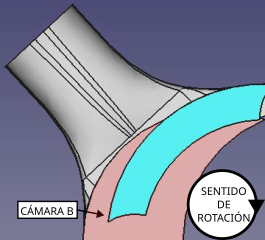
\includegraphics[width=\textwidth]{flujometrias/sin_solape.png}
        \caption{Sin solape}
    \end{subfigure}%
    \begin{subfigure}[t]{0.4\textwidth}
        \centering
        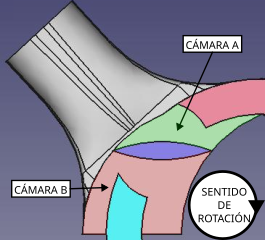
\includegraphics[width=\textwidth]{flujometrias/con_solape.png}
        \caption{Con solape}
    \end{subfigure}
  \caption{Solape de cámaras}\label{fig:solape}
\end{figure}

Independientemente del tipo de flujo que se esté simulando, de ICESym se toman
los valores de presión, temperatura, densidad y velocidad para calcular los
valores iniciales.

Debido a la cantidad de flujometrías a realizar, se utilizó un \emph{script} para leer
los datos de salida de ICESym y calcular los valores requeridos en función del
tipo de flujo a simular.
%
Este \emph{script} toma el estado del gas del simulador tanto en la cámara de
combustión como del puerto que se esté analizando, para la posición de alzada y
RPM requeridas.
%
Con estos valores se calculan las propiedades termodinámcicas del gas con las
siguientes relaciones para cada cámara analizada, los valores leídos son:

\begin{itemize}
    \item $\rho_{c,i}$, es la densidad del gas en la cámara de combustión $i$.
    \item $P_{c,i}$, es la presión del gas en la cámara de combustión $i$.
    \item $T_{c,i}$, es la temepratura del gas en la cámara de combustión $i$.
    \item $\rho_{p,i}$, es la densidad del puerto $i$.
    \item $v_{p,i}$, es la velocidad del gas en el puerto $i$.
    \item $P_{p,i}$, es la presión del gas en el puerto $i$.
\end{itemize}

Con estos valores iniciales se pueden calcular o estimar las propiedades
termodinámicas de la mezcla de gases frescos o quemados, dependiendo si se está
evaluando un puerto de admisión o escape, los valores calculados son:
%
\begin{itemize}
    \item $M_{M}$, Masa molar, ec.\ref{eq:mw}
    \item $C_{p}$, Calor específico a presión constante.
    \item $\gamma$, Relación $C_{p}/C_{v}$ del gas
    \item $\mu$, Viscosidad dinámica, ec.\ref{eq:mu}
    \item $\nu$, Viscosidad cinemática
    \item $P_{R}$, Número de Prandtl, ec\ref{eq:pr}
    \item $k_{est}$, Energía cinética turbulenta, ec.\ref{eq:kappa_est}
    \item $\epsilon_{est}$, Disipación de la energía cinética turbulenta, ec.\ref{eq:epsilon_est}
\end{itemize}

Para simplificar el análisis no se tuvo en cuenta la fracción de gases
residuales, el gas ``flujado'' es siempre aire limpio en el caso de los puertos
de admisión o el gas quemado de una mezcla estequeométrica de aire-combustible
en caso de los puertos de escape, siendo isooctano $C_{8}H_{18}$ el combustible
seleccionado.
%
Las ecuaciones utilizadas para modelar las propiedades termodinámicas de las
mezclas aire-combustible fueron descritas brevemente en la
sección~\ref{subsec:prop_mezcla}.

\subsection{Malla}

La malla se construyó a partir del modelo de CAD generado con los resultados
obtenidos de las simulaciones del motor.
%
La implementación de las diferentes herramientas requeridas para generar una
malla apta para realizar las flujometrías se describe en el
apartado~\ref{sec:cap3_of_malla}.

El grado de refinamiento de la misma se determinó luego de realizar una serie de
flujometrías con tamaños decrecientes de celda y viendo la variabilidad de los
resultados.
%
El objetivo de las flujometrías es obtener el flujo másico $\dot{m}$ del puerto
para un estado del gas dado, se redujo el tamaño inicial de celda hasta que el
valor de $\dot{m}$ no se modificó en más de un 5\% del valor anterior, con un
nivel de refinamiento mayor.
%
En algunos casos se utilizaron los resultados de flujometrías con mallas menos
refinadas como valor inicial de una malla de mayor refinamiento, esto con el
propósito de reducir el tiempo de simulación de las mallas con mayor número de
celdas.
%
Por ejemplo, con una malla inicial de cubos de 15mm de lado se obtiene una
solución que se usa como valor inicial para una malla de 10mm, a su vez este
resultado se utiliza como valor inicial de la simulación final con una malla de
cubos de 5mm de lado para obtener el valor de $\dot{m}$ utilizado para calcular
el $C_{D}$.

\subsection{Coeficiente de descarga $C_{D}$}\label{sec:cap2_cd}

El flujo másico que circula a través del puerto se calcula a partir de las
ecuaciones de flujo compresible a través de una restricción, habiendo dos casos
distintivos: flujo bloqueado y no bloqueado.

El flujo está bloqueado si la velocidad en la garganta de la restricción alcanza
la velocidad sónica, dada esta condición el flujo másico alcanza un límite y
reducir la presión aguas abajo de la restricción no produce un aumento del caudal.
%
La condición de flujo bloqueado se puede expresar en términos de la relación de
presiones aguas arriba $p_{0}$ y aguas abajo de la restricción $p_{T}$.
%
Si se cumple la inecuación~\ref{eq:condicion_bloqueo}, el flujo está bloqueado.

El caudal másico para la condición de flujo no bloqueado se calcula con la
ecuación~\ref{eq:m_no_bloqueo} y la ecuación~\ref{eq:m_bloqueo} en caso de que
esté bloqueado.
%
Los parámetros involucrados en estas ecuaciones son:
\begin{itemize}
    \item $p_0$, es la presión de estancamiento antes de la restricción.
    \item $T_0$, es la temperatura de estancamiento antes de la restricción.
    \item $p_T$, es la presión estática justo después de la restricción.
    \item $A_R$, es el área de referencia.
    \item $\dot{m}$, es el caudal másico.
    \item $\gamma$, es el cociente de capacidades térmicas del gas.
\end{itemize}

\begin{equation}\label{eq:condicion_bloqueo}
  \frac{p_{T}}{p_{0}} \le {\left(\frac{2}{\gamma+1}\right)}^{\frac{\gamma}{\gamma - 1}}
\end{equation}

\begin{equation}
    \label{eq:m_no_bloqueo}
    \dot{m} = \frac{C_D A_R p_0}{\sqrt{R T_0}}
            {\left(\frac{p_T}{p_0} \right)}^{1/\gamma}
            {\left( \frac{2\gamma}{\gamma-1} \left[1- {\left(\frac{p_T}{p_0}\right)}^{{\gamma-1}/\gamma} \right] \right)}^{1/2}
\end{equation}

\begin{equation}\label{eq:m_bloqueo}
  \dot{m}=  \frac {C_D A_R p_0} {{(R T_0)}^{1/2}}
            \gamma^{1/2}
            {\left( \frac{2\gamma}{\gamma+1} \right)}^{(\gamma+1)/(2(\gamma-1))}
\end{equation}

Un parámetro importante en las ecuaciones anteriores es el área de referencia
$A_{R}$, define el área utilizada para calcular el caudal másico que circula por
el puerto.
%
En un motor con válvulas se suele tomar el área de cortina como el producto de
la circunferencia de la válvula con la alzada, es decir

\begin{equation}\label{eq:ar_cortina}
  A_{R}=\pi D_{v} \cdot h_{v}
\end{equation}

El área de referencia utilizada en ICESym es el área frontal del puerto expuesta
a la cámara que se esté analizando, calculada como

\begin{equation}\label{eq:ar_mrcvc}
  A_{R} = h_{p} \cdot l_{v}
\end{equation}

El área de cortina se ilustra en la figura~\ref{fig:area_cortina} y el área
utilizada en ICESym para el MRCVC en la figura~\ref{fig:area_referencia}.
%
En esta última figura se observan dos zonas coloreadas, que hacen referencia al
área de dos cámaras durante el solape de cámaras que ocurre en el puerto.

\begin{figure}[ht]
    \centering
    \begin{subfigure}{0.5\textwidth}
      \centering
      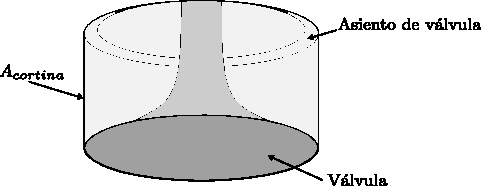
\includegraphics[width=\textwidth]{valve_curtain.pdf}
      \caption{Área de cortina}\label{fig:area_cortina}
    \end{subfigure}%
    \begin{subfigure}{0.5\textwidth}
      \centering
      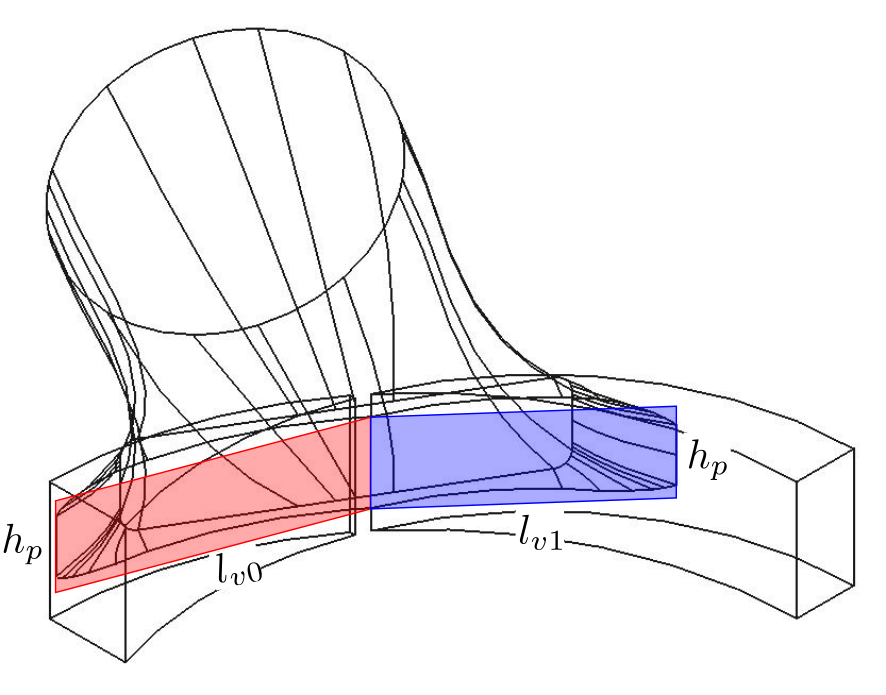
\includegraphics[width=\textwidth]{area_referencia.png}
      \caption{Área de referencia MRCVC}\label{fig:area_referencia}
    \end{subfigure}
    \caption{Área de referencia}
\end{figure}

Los valores de densidad, velocidad, presión y temperatura se obtienen de los
datos de salida de ICESym para un puerto, ángulo y velocidad dada.
%
Para la temperatura se utiliza la temperatura de cámara, $T_0 = T_C$, la presión
antes y después del puerto se selecciona de acuerdo al sentido de flujo, en caso
de ser hacia la cámara de combustión la presión en el puerto se utiliza como
inicial $P_0$ y la presión en la cámara es la aproximación a la presión en la
restricción $P_T$.

El valor de $\gamma$ se obtiene de las propiedades de la mezcla con las rutinas
computacionales descritas en el apartado~\ref{subsec:prop_mezcla}.

De las flujometrías se obtiene el caudal másico que fluja el puerto, con este
dato y las ecuaciones anteriores se puede determinar el valor de $C_{D}$.

% \subsection{otro}


% Para inicializar el campo de presión y densidades, se usa la media entre las
% cámaras que se estén simulando y se establece un campo uniforme.

% La velocidad se inicializa con un campo nulo de velocidades, que en la
% configuración de OpenFOAM se designa como \emph{internalField uniform (0 0 0)}.

% En resumen, los valores iniciales de los campos de presión, temperatura y velocidad
% son los indicados en la tabla~\ref{tab:cc}.

% % \begin{table}
% % \centering
% %     \begin{tabular}{cccc} \toprule
% %         Var & Campo         & Parche                      & Pared \\
% %         T   & uniforme T0   & inletOutlet                 & uniforme T9\\ \midrule
% %         P   & uniform Pavg  & uniformTotalPressure        & Pi \\
% %         U   & uniform (0 0 0) & pressureInletOutletVelocity & valor fijo (0 0 0)\\
% %         rho & uniform rhoAvg \\ \bottomrule
% %     \end{tabular}
% %     \caption{Condiciones de Borde}\label{tab:cc}
% % \end{table}

% En todos los casos se tomará como velocidad de referencia a la media entre la
% velocidad en la punta del tubo de las cámaras solapadas.
% %
% Del mismo modo, la temperatura será la temperatura de cámara media.

% Si hay o no solape de cámaras va a depender tanto de la geometría del puerto
% como de la posición del ciclo en la que se encuentre, para determinar las
% condiciones iniciales se debe tener en cuenta el solape.
% %
% En la figura~\ref{fig:geom} se muestra un corte del puerto con un plano cuya
% normal está en $\vec{z}$, se denominará a la cámara que esté a la izquierda
% como cámara 0 y a la que esté a la derecha cámara 1.
% %
% Al haber solape de cámaras, para definir la presión del puerto y estimar las
% condiciones iniciales de los parámetros viscosos que requiere el modelo
% $k-\epsilon$ se utilizan valores medios de presión, velocidad y temperatura de
% ambas cámaras.
% %
% Además, las condiciones iniciales que se aplican al parche denominado
% \emph{puerto} es igual a la media aritmética de la velocidad de las velocidades
% de los puertos de ambas cámaras, Lo mismo sucede con la presión, densidad y
% temperatura.

% A partir de estos datos se calculan varias propiedades termodinámicas del gas,
% incluyendo la constante del gas, masa molar, viscosidad cinemática y demás.
% %
% Para calcular estas propiedades se asume que el gas no contiene gases
% residuales.

% Finalmente el caudal másico yse obtiene con OpenFOAM, en donde se simula el
% tiempo suficiente para que los caudales másicos por entradas o salidas se
% estabilice, como se ve en la figura~\ref{fig:caudalMasico}.

% \begin{figure}
%     \centering
%     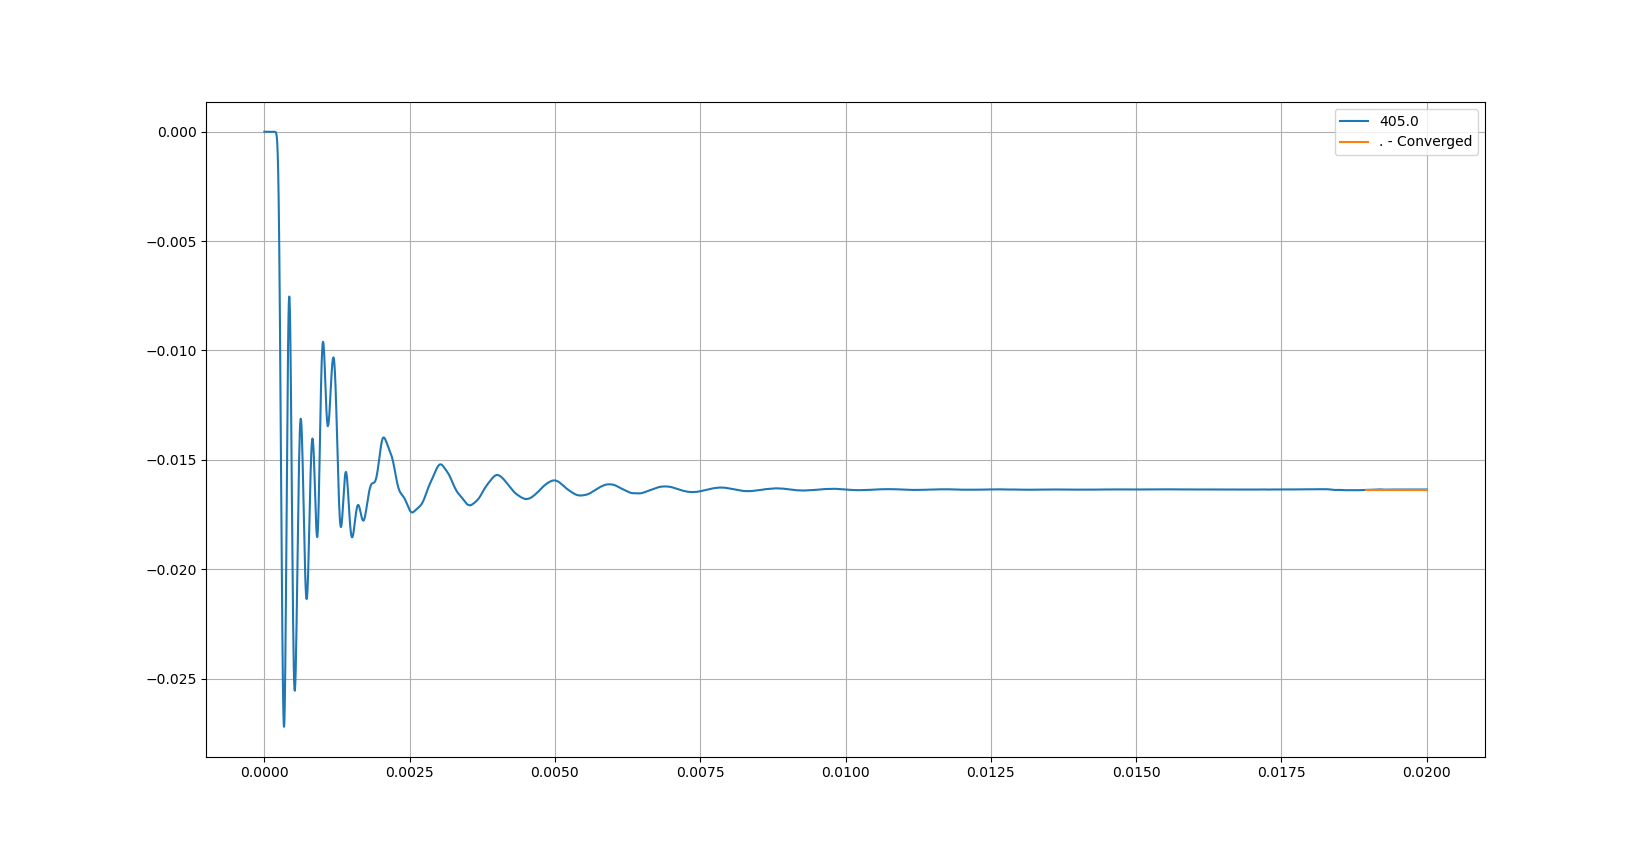
\includegraphics[width=0.6\textwidth]{surfaceFieldValue_405.0.png}
%     \caption{Flujometrías para el puerto de Admisión}\label{fig:caudalMasico}
% \end{figure}

% En todos los casos se tomará como velocidad de referencia a la media entre la
% velocidad en la punta del tubo de las cámaras que se estén solapando.
% %
% Del mismo modo, la temperatura será la temperatura de cámara media.

% Si hay o no solape de cámaras va a depender tanto de la geometría del puerto
% como de la posición del ciclo en la que se encuentre, para determinar las
% condiciones iniciales se debe tener en cuenta el solape.
% %
% En la figura~\ref{fig:geom} se muestra un corte del puerto con un plano cuya
% normal está en $\vec{z}$, se denominará a la cámara que esté a la izquierda
% como cámara 0 y a la que esté a la derecha cámara 1
% %
% Al haber solape de cámaras, para definir la presión del puerto y estimar las
% condiciones iniciales de los parámetros viscosos que requiere el modelo
% $k-\epsilon$ se utilizan valores medios de presión, velocidad y temperatura de
% ambas cámaras.
% %
% Además, las condiciones iniciales de que se aplican al parche denominado
% \emph{puerto} es igual a la media aritmética de la velocidad de las velocidades
% de los puertos de ambas cámaras, Lo mismo sucede con la presión, densidad y
% temperatura.
